\subsection{Luminosity and Cross Section}

In this dissertation we are measuring the total and the differential cross section. Fig.~\ref{fig:CSclassical} illustrates the concept of the differential cross section in the classical case. An incident particle must appear within area $d\sigma$ to be scattered off by an angle $d\theta$ by the scattering center. The relashionship between these two quantities would give us the expression for the differential cross section $d\sigma/d\theta$. Integrating over $d\theta$, one would get the total cross section $\sigma$. Differentiating $\sigma$ by any kinematic parameter $X$ of the incident particle would give the expression for the differential cross section $d\sigma/dX$.\\

\begin{figure}[htb]
  \begin{center}
    {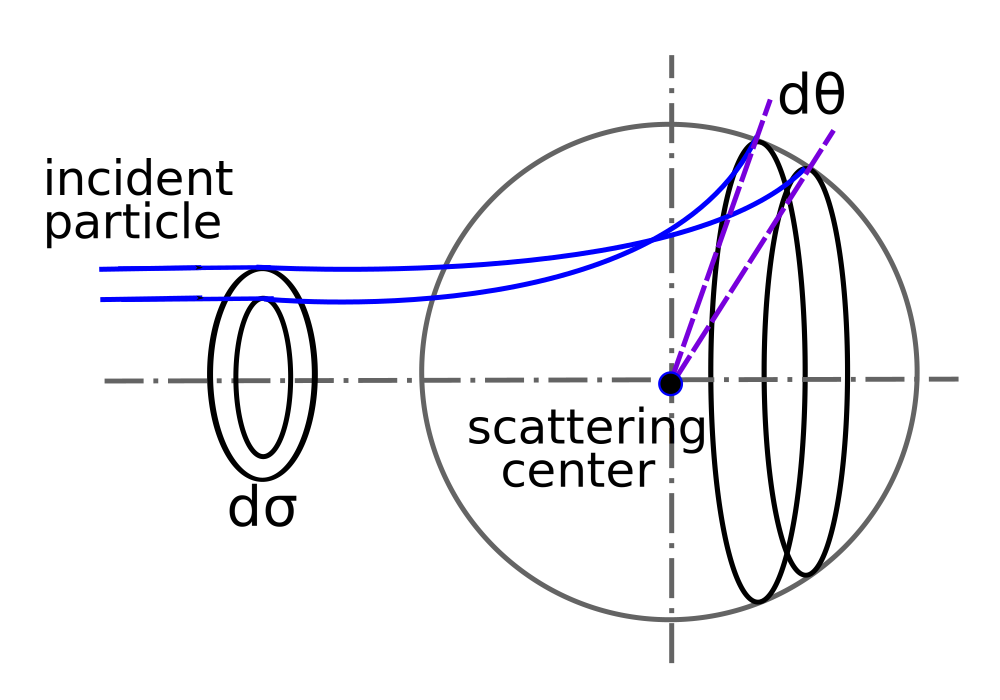
\includegraphics[width=0.70\textwidth]{../figs/WgAbout/CSclassical.png}}
    \caption{Illustration of the differential cross section concept in the classical case.}
    \label{fig:CSclassical}
  \end{center}
\end{figure}


In particle physics the cross section characterizes the probability of two particles to interact \cite{ref_Griffiths}, \cite{ref_Halzen_Martin}, \cite{ref_CS_wiki} or, more specifically, the probability of two particles to interact to produce the specific final state. For example, the probability of a quark and an antiquark to interact to produce a charged lepton, a neutrino and a photon like in our measurement.\\

Referring to the Fig. \ref{fig:CSclassical}, a number of particles passing through the area $\sigma$ per unit time is $N=L \cdot \sigma$, where L is the number of particles crossing the unit area integrated over a period of time when $N$ events occur. Therefore, the cross section $\sigma$ of a specific process $\sigma=N/L$ where N is a number of events of the process occurred. $L$ in this expression refers to the number of the initial state particles and is called the luminosity. \\
  
%Thus, to measure the cross section we need to know total number of events of the given process but we cannot detect events which are out of the detector acceptance or which do not fall satisfy analysis selection criteria. Therefore, the number of events $N$ has to be corrected in a measurement: $N \rightarrow N/(A \cdot \epsilon)$, where $A$ is a detector acceptance and $\epsilon$ is an efficiency of a signal process to pass selection criteria. Other corrections to $N$ may have to be applied depending on the analysis.\\

%The luminosity $L$ is determined based on the collider characteristics. $L$ may not be uniform in time however we are usually interested in measuring the total or differential cross section as a function of a certain kinematic parameter of a final state particle or of a system of final state particles rather than the differential cross section as a function of time and therefore integrate the luminosity over the period of time.\\

% Add more from Griffiths

To compute a cross section theoretically, one has to know the amplitude of the process $M$  (Chapter \ref{sec:WgAbout_SMproduction}, \cite{ref_Griffiths}) and the phase space. The formula of the cross section is called the Fermi's Golden rule \cite{ref_Griffiths}. In case of the scattering of two particles to three final state particles $1+2\rightarrow 3+4+5$, it takes the following form:\\

\begin{equation}\label{eq:FermiGoldenRule}
\sigma = \frac{ \hbar^2 }{4\sqrt{(p_1p_2)^2-(m_1m_2c^2)^2}} \int |M|^2 (2\pi)^4 \delta^4(p_1+p_2-p_3-p_4-p_5) \prod_{j=3}^{5} \frac{1}{2 \sqrt{\bar{p_j^2}+m_j^2 c^2}}\frac{d^3\bar{p_j}}{(2\pi)^3}  
\end{equation}

where $\hbar$ is the Planck constant, $c$ is the speed of light, $p_i$ are 4-momenta and ${\bar{p_i}}$ are three momenta of the initial state and the final state particles, $m_i$ are masses of particles.\\ 

The calculation of the process amplitude starts with writing the relevant Lagrangian similarly to how it is done in the classical mechanics but in particle physics instead of coordinates we have quantum fields. The Lagrangian allows us to derive the equations of motion however they cannot be solved exactly and, therefore, the perturbative approach is used if coupling constants are $g \ll 1$.\\

%Consider discussing parton luminosity and the cross section expression that involves the PDFs and parton-based cross sections

In case of the proton-proton collisions, we can factorize a cross section of a process $pp \rightarrow P+X$ to a partonic cross section $\sigma(ij \rightarrow P)$ and parton distribution functions $f_i(x_1,Q^2)$ \cite{ref_PDG}, \cite{ref_Lindsey_thesis}:\\

\begin{equation}\label{eq:ppCS_general}
  \sigma(pp \rightarrow P+X)= \sum_{i,j} \int dx_1 dx_2 f_i(x_1,Q^2) f_j(x_2, Q^2) \sigma(ij \rightarrow P).
\end{equation}

In case of $W\gamma$ process, Eq.~\ref{eq:ppCS_general} takes the following form: \\
%$ij$ can be any $q_1 \bar{q}_2$ pair such that the total charged of $q_1$ and $\bar{q}_2$ equals $\pm 1$.\\

\begin{equation}\label{eq:ppCS_Wg}
  \sigma(pp \rightarrow l \nu_l \gamma + X)= \sum_{i,j} \int dx_1 dx_2 f_i(x_1,Q^2) f_j(x_2, Q^2) \sigma(q_i \bar{q}_j \rightarrow l \nu_l \gamma).
\end{equation}

